В этой главе собраны некоторые общие знания о типах.

Разделы~\ref{subsec:variance}, ~\ref{subsec:isomorphism} в основном следуют~\cite[глава 1]{maguire-types}.

\subsection{Полярности и вариантность} \label{subsec:variance} % todo

В этом параграфе мы будем рассматривать тему с точки зрения программирования~\cite[глава 3]{maguire-types}, не отдавая должного теории категорий.
Восполнить пробел можно с помощью замечательной статьи, написанной в жанре пьесы~\cite{hinze2012functional}.

\vocab{Ковариантный функтор} --- пара из типового конструктора \texttt{F} и операции на функциях \texttt{fmap :: (a -> b) -> (F a -> F b)}.
Плюс законы о том, что \texttt{fmap} уважает \texttt{id} и композицию.

\begin{minted}{haskell}
    class Functor f where
      fmap :: (a -> b) -> (f a -> f b)
\end{minted}

\begin{figure}[H]
    \centering
    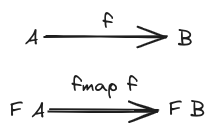
\includegraphics[width=0.3\textwidth]{figs/functor}
\end{figure}

\vocab{Контравариантный функтор} --- пара из типового конструктора и операции на функциях, разворачивающей стрелку.
Плюс соответствующие законы.

\begin{minted}{haskell}
    class Contravariant f where
      contramap :: (a -> b) -> (f b -> f a)
\end{minted}

\begin{figure}[H]
    \centering
    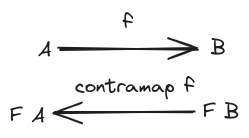
\includegraphics[width=0.3\textwidth]{figs/contra-functor}
\end{figure}

Типовой конструктор можно объявить ковариантным или контравариантным функтором (или никаким из них) относительно типового параметра в зависимости от вида декларации соответствующих конструкторов данных.
А именно, от \vocab{полярности}\footnote{\url{https://existentialtype.wordpress.com/2012/08/25/polarity-in-type-theory/}}\footnote{\url{https://ncatlab.org/nlab/show/polarity+in+type+theory}} позиций, в которых входит этот типовой параметр.

Попробуем развить интуитивное понимание полярностей.
Рассмотрим некоторое вычисление типа \texttt{F a}.
Параметр \texttt{a} входит в положительной позиции, если все его значения можно извлечь из \texttt{F a}, как в следующих примерах (для извлечения могут понадобиться паттерн-матчинг и аппликация):
\begin{minted}{haskell}
    data F a = L a | R a
    data F a = D a (Int -> a)
\end{minted}

Вхождения, наоборот, отрицательные, если значения соответствующего типа нельзя получить из вычисления, но нужно ему предоставить.
Например, в качестве параметров функций:
\begin{minted}{haskell}
    data F a = F (a -> Int)
    data F a = L (a -> ()) | R Int
\end{minted}
Действительно, для первого примера можно объявить инстанс \mintinline{haskell}|Contravariant|:
\begin{minted}{haskell}
    instance Contravariant F where
      contramap :: (a -> b) -> (F b -> F a)
      contramap g (F f) = F (f . g)
\end{minted}

Можно предположить, что на плюс и минус действуют обычные мультипликативные законы.
И это действительно так.
\begin{itemize}
    \item Плюс на плюс даёт плюс:
    \begin{minted}{haskell}
        data F a = F (Int -> (Int -> a))
    \end{minted}
    \item Плюс на минус (и наоборот) --- минус:
    \begin{minted}{haskell}
        data F a = F ((Int -> a) -> Int)
    \end{minted}
    \item Минус на минус --- плюс, поскольку параметр принимаемой функции выдаётся реализацией вызывающей стороне:
    \begin{minted}{haskell}
        data F a = F ((a -> Int) -> Int)
    \end{minted}
\end{itemize}

Тип от двух положительных параметров можно объявить \vocab{бифунктором}:
\begin{minted}{haskell}
    class Bifunctor f where
      bimap :: (a -> c) -> (b -> d) -> f a b -> f c d
\end{minted}

Тип от двух параметров, положительного и отрицательного, --- \vocab{профунктором}:
\begin{minted}{haskell}
    class Profunctor p where
      dimap :: (c -> a) -> (b -> d) -> p a b -> p c d
\end{minted}

Профункторы являются некоторыми обобщениями функциональной стрелки.
Например, если у нас есть SQL запрос, который по данным возвращает результат, его можно объявить профунктором с семантикой --- добавить пред-обработку входных данных и пост-обработку выходных:
\begin{minted}{haskell}
    dimap serialize deserialize (query :: Sql Text Text) :: Sql Age [User]
\end{minted}

Также понятие вариантности часто встречается в объектно ориентированных языках для обозначения возможности дополнить отношение подтипизации на полиморфные типы (да и вообще в теории подтипизации).

Действительно, \vocab{отношение подтипизации} \texttt{B <: A} говорит о том, что значение типа \texttt{B} безопасно использовать в позиции, где ожидается значение типа \texttt{A}.
Иначе говоря, существует функция \texttt{upcast :: B -> A}.
Если типовой конструктор \texttt{F a} ковариантен относительно параметра \texttt{a}, то по \texttt{upcast} найдётся \texttt{upcast' :: F B -> F A}.
То есть отношение подтипизации также автоматически включает \texttt{F B <: F A}.
Контравариантный случай аналогично.

\begin{task}
    Убедитесь в вашем любимом языке с поддержкой вариантности, что минус на минус даёт плюс.
\end{task}

\subsection{Изоморфизм} \label{subsec:isomorphism}

Мы будем придерживаться теоретико-множественной интерпретации типов.
С категорным взглядом на происходящее можно ознакомиться в~\cite{hinze2010reason}.

Пусть нам нужно спроектировать функцию или модель данных.
Мы начинаем с декларации типа, как её выбрать и из каких вариантов?
Для начала поймём, когда два типа взаимозаменимы, для этого рассмотрим понятия изоморфизма.

Два типа \texttt{A} и \texttt{B} называются \vocab{изоморфными} (обозначают \texttt{A $\iso$ B}) тогда и только тогда, когда существует такая пара функций \texttt{to :: A -> B} и \texttt{from :: B -> A}, что\footnote{Под равенством термов можно понимать разное, например, $\alpha\beta\gamma$-эквивалентность. Мы будем пользоваться \vocab{экстенсиональным равенством} для функций~--- две функции равны, когда равны их результаты на всех входах. \url{https://ncatlab.org/nlab/show/function+extensionality}}
\begin{minted}{c}
    to . from = id
    from . to = id
\end{minted}

Иначе говоря, между обитателями таких типов можно установить взаимно-однозначное соответствие.
Легко понять, что со смысловой точки зрения не принципиально, какой из изоморфных типов использовать --- их можно заменять друг на друга добавляя вызовы функций перехода.
Такие два типа заключают в себе одинаковое ``количество информации''.
Например, типы \mintinline{haskell}|Bool| и \mintinline{haskell}|Maybe ()| в этом смысле совершенно взаимозаменимы.
Покажем это, предъявив пару взаимообратных функций\footnote{Нужно не забыть показать взаимообратность функций, но это делается тривиально перебором входов (может быть с помощью индукции) и редукцией.}:
\begin{minted}{haskell}
    to :: Bool -> Maybe ()
    to b = if b then Just () else Nothing

    from :: Maybe () -> Bool
    from m = case m of Nothing -> False; Just () -> True
\end{minted}

Несмотря на смысловую взаимозаменимость, для кодирования информации о том, передал ли пользователь программе определённый флаг, мы, скорее всего, воспользуемся типом \mintinline{haskell}|Bool| ввиду нефункциональных соображений о читабельности кода.
Аналогично можно рассматривать соображения эффективности.

\subsubsection{Кардинальность: суммы, произведения, экспоненты} \label{subsubsec:cardinality}

Типы можно воспринимать как синтаксис для записи множеств, а населяющие их термы~--- как синтаксические записи элементов этих множеств.
Так терм \mintinline{haskell}|(True, False)|~--- запись элемента множества пар, записываемого в синтаксисе типов как \mintinline{haskell}|(Bool, Bool)| (вместо математического $\mathbb{B}\times\mathbb{B}$).
Или же терм \mintinline{haskell}|\x -> x + 1| является записью функции прибавляющей единицу из множества функций над целыми числами, записываемого как \mintinline{haskell}|Integer -> Integer| (вместо математического $\mathbb{Z}\to\mathbb{Z}$).

Заметим, что два типа изоморфны, если соответствующие им множества имеют одинаковое количество элементов.
Более того, таких изоморфизмов $n!$ в случае конечности множеств.
Научимся определять количество таких элементов.
С помощью $|\cdot|$ будем записывать \vocab{кардинальность} типа~--- количество элементов в соответствующем множестве.

\begin{center}
    \begin{tabular}{|l|c|}
        \hline
        Тип и его декларация                                                                                                                                                                            & кардинальность \\
        \hline
        \mintinline{haskell}{data Void}                                                                                                                                                                 & $0$            \\
        \mintinline{haskell}{data Unit = Unit}\footnote{\mintinline{haskell}|Unit| записывается в Haskell с помощью специального синтаксиса \mintinline{haskell}|()|, означающем как бы пустой кортеж.} & $1$ \\
        \mintinline{haskell}{data Bool = False | True}                                                                                                                                                  & $2$            \\
        \hline
    \end{tabular}
\end{center}

Идея алгебраических типов данных в том, что сложные типы можно строить из простых с помощью операции $+$ (``или'') и операции $\times$ (``и'')\footnote{\url{https://stanford-cs242.github.io/f18/lectures/02-2-algebraic-data-types.html}}:
\begin{center}
    \begin{tabular}{|l|c|}
        \hline
        Тип                                                      & кардинальность   \\
        \hline
        \mintinline{haskell}{data Either a b = Left a | Right b} & $|a| + |b|$      \\
        \mintinline{haskell}{data Pair a b = Pair a b}           & $|a| \times |b|$ \\
        \hline
    \end{tabular}
\end{center}

Посчитаем количество обитателей различных типов (вы можете убедиться в справедливости заключения перебрав все термы вручную):
\begin{itemize}
    \item \mintinline{haskell}{|Either Unit (Eigher Bool Bool)| = |Unit| + (|Bool| + |Bool|) = 5}.
    \item \mintinline{haskell}{Pair (Either Bool Unit) (Pair Unit Void)| = 0} ~--- тип \mintinline{haskell}|Void| не населён, как и кортеж, его включающий.
    \item Если \mintinline{haskell}{data Example = FirstAlternative Bool | AnotherOne Unit Bool Bool}, то \\\mintinline{haskell}{|Example| = |Bool| + |Unit| * |Bool| * |Bool| = 2 + 1 * 2 * 2 = 6}.
\end{itemize}

Функциональную стрелку называют экспоненциальным типом.
Действительно, комбинаторно количество обитателей \mintinline{haskell}|A -> B| вычисляется как \[|A \to B| = |B|^{|A|}\]

Так как проектировать типы?
Тому есть несколько соображений:
\begin{itemize}
    \item В типе должно быть не меньше элементов, чем в предметной области, все необходимые объекты были представимы.
    \item В типе должно быть как можно меньше элементов, которых нет в предметной области, чтобы пространство ошибок было минимальным.
    \item Далее среди изоморфных типов выбирается оптимальный исходя из функциональных и нефункциональных требований.
\end{itemize}

Прежде чем работать с некоторым объектом предметной области, информацию о нём, в соответствии со вторым правилом, следует привести в максимально структурное представление, дающее наибольшее количество гарантий\footnote{\url{https://lexi-lambda.github.io/blog/2019/11/05/parse-don-t-validate/}}.

\subsubsection{Алгебраическое представление типа} \label{subsubsec:type-algebra}

Как мы увидели выше, чтобы показать наличие изоморфизма между двумя типами можно либо предъявить пару взаимообратных функций, либо показать, что кардинальности этих двух типов совпадают.
В этом разделе мы научимся сопоставлять типу некоторую алгебраическую запись, отражающую его структуру и кардинальность.
Так, мы сможем синтаксическими преобразованиями формул получать эквивалентные записи, из которых будем восстанавливать типы, заведомо изоморфные данному\footnote{\url{https://codewords.recurse.com/issues/three/algebra-and-calculus-of-algebraic-data-types}}.

В основу алгебраического представления положим вычисление кардинальности типов:
\begin{center}
    \begin{tabular}{|p{0.5\textwidth}|c|}
        \hline
        Тип                                                      & алгебраическая формула      \\
        \hline
        \mintinline{haskell}{data Void}                          & $0$                         \\
        \mintinline{haskell}{data Unit = Unit}                   & $1$                         \\
        \mintinline{haskell}{data Bool = False | True}           & $1 + 1$ (обозначим как $2$) \\
        \mintinline{haskell}{data Maybe a = Nothing | Just a}    & $1 + a$                     \\
        \mintinline{haskell}{data Either a b = Left a | Right b} & $a + b$                     \\
        \mintinline{haskell}{data Pair a b = Pair a b}           & $a \times b$                \\
        \mintinline{haskell}{a -> b}                             & $b^a$                       \\
        \hline
    \end{tabular}
\end{center}

\begin{task}
    Запишите в алгебраическом виде следующий тип:
    \begin{minted}{haskell}
        data T a b = Undefined | Defined a (a -> b)
    \end{minted}
\end{task}

В качестве отношения эквивалентности, будем использовать изоморфизм соответствующих типов.
В такой интерпретации, классические свойства операций сохраняются (рис.~\ref{fig:school-alg}).
Действительно, например:
\begin{minted}{haskell}
    -- ?$(c^b)^a \iso c^{a\times b}$?
    to :: (a -> b -> c) -> (a, b) -> c
    to = uncurry
    from :: ((a, b) -> c) -> a -> b -> c
    from = curry
\end{minted}

\begin{figure}
    \centering
    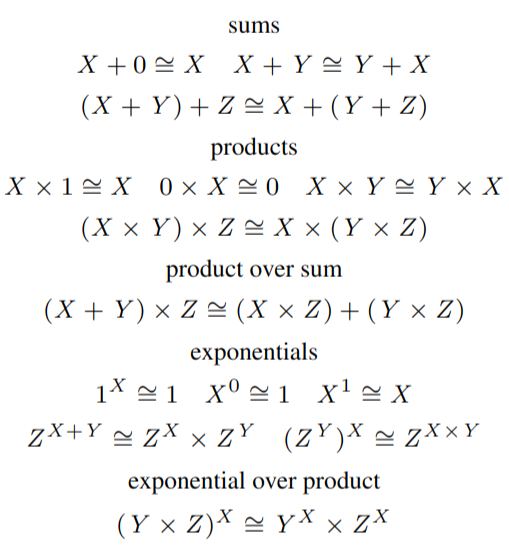
\includegraphics[width=0.4\textwidth]{figs/school-alg}
    \caption{Законы школьной алгебры ностальгии ради~\cite{hinze2010reason}.}
    \label{fig:school-alg}
\end{figure}

\begin{task}
    Покажите, что $(a + b) + c \iso a + (b + c)$.
\end{task}

\begin{task}
    Покажите, что $c^{a + b} \iso c^a\times c^b$.
\end{task}

Интересным наблюдением может быть то, что функции можно использовать как структуры данных, в соответствие с изоморфизмом $c^{a + b} \iso c^a\times c^b$.
Действительно, в таком случае аргумент функции выступает индексом (его кардинальность должна совпадать с размером коллекции).
Это очень важный изоморфизм, мы к нему вернёмся, чтобы проложить путь к tagless-final интерпретаторам и коданным в главе~\ref{sec:wonder-interpreters}.
\begin{minted}{haskell}
    -- ?$a \times a \iso a^2$?
    get :: (a, a) -> (Bool -> a)
    get (x, y) idx = if idx then x else y
    tabulate :: (Bool -> a) -> (a, a)
    tabulate f = (f True, f False)
\end{minted}

\vocab{Каноническим предствлением типа (canonical representaion)} называют сумму произведений типов:
\[
    \sum_{i}\prod_{j} t_{ij}
\]
Каноническое представление является своего рода нормальной формой, в которой можно записывать алгебраические типы (любой алгебраический тип можно по правилам привести к ней).
Легко узнать в нём вид \mintinline{haskell}{data} деклараций в Haskell.
В дальнейшем мы воспользуемся каноническим представлением для обобщённой работы с типами (глава.~\ref{sec:datatype-generic}).

\subsection{Рекурсивные типы и схемы} \label{subsec:recursive-types}

TODO % todo

\subsection{Немного категорий} \label{subsec:cats}

TODO % todo
